\section{Performances}
\label{sec:performances}

\begin{figure}[t!]
	\centering
	\centering
	\includegraphics[width=\columnwidth]{figures/plots/realistic_tr}
	\caption{Throughput of the different protocols in respect to the total load on the channel with the realistic propagation model. Simple Carrier Sensing performs better then Trivial Carrier Sensing and Aloha. The highest throughput is obtained at \SI{10}{Mbps} of load. When the load is higher, the performances of all protocols tend to zero.}
	\label{fig:tr}
\end{figure}

\begin{figure}[t!]
	\centering
    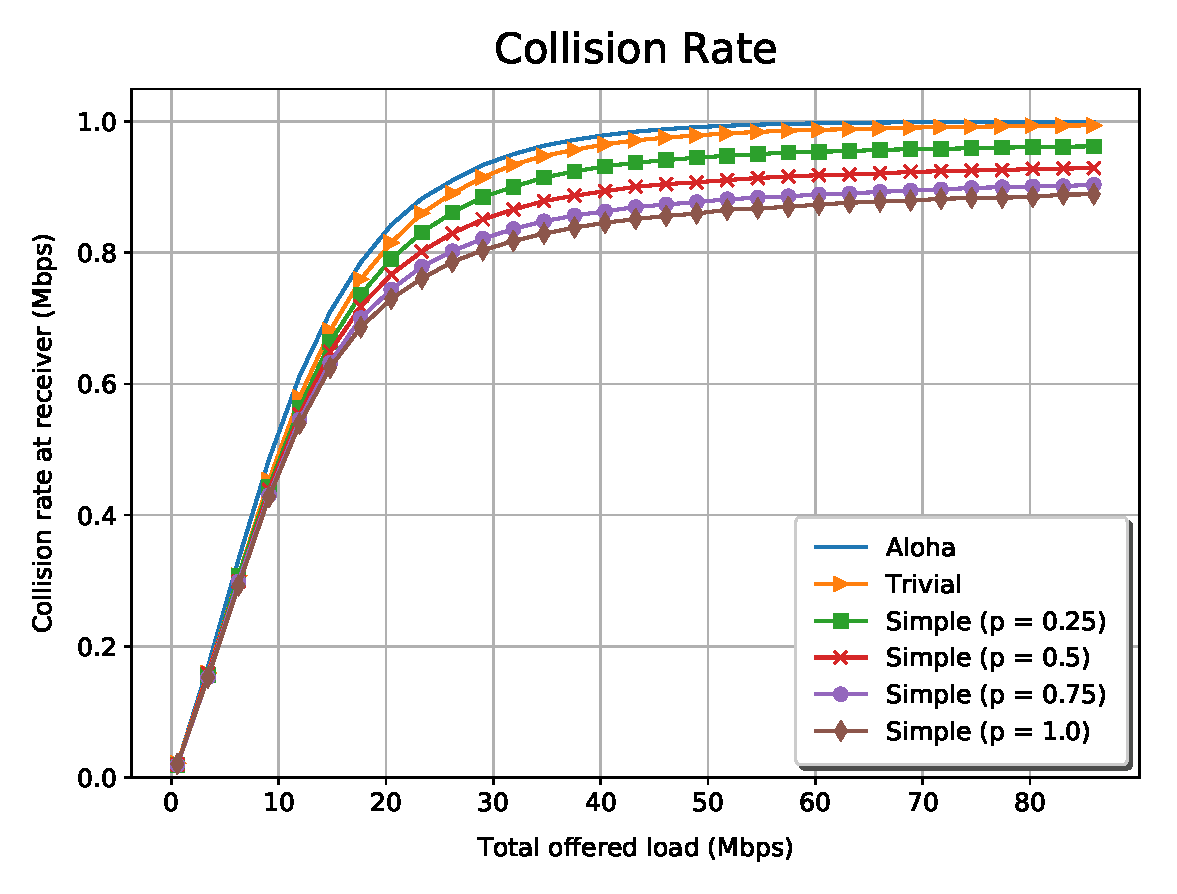
\includegraphics[width=\columnwidth]{figures/plots/realistic_cr}
	\caption{Collision Rate of the different simulations with respect to the total offered load. High collision rates degrade the performances of the protocol. Aloha and Trivial Carrier Sensing have the higher collision rate.}
	\label{fig:cr}
\end{figure}

\begin{figure}[t!]
	\centering
    \includegraphics[width=\columnwidth]{figures/plots/realistic_dr}
	\caption{Packet Drop Rate at the sender for the realistic propagation model. Aloha has a packet drop rate significantly lower then the other protocols, while there is not big difference between Simple and Trivial Carrier Sensing.}
	\label{fig:dr}
\end{figure}

\begin{figure}[t!]
	\centering
    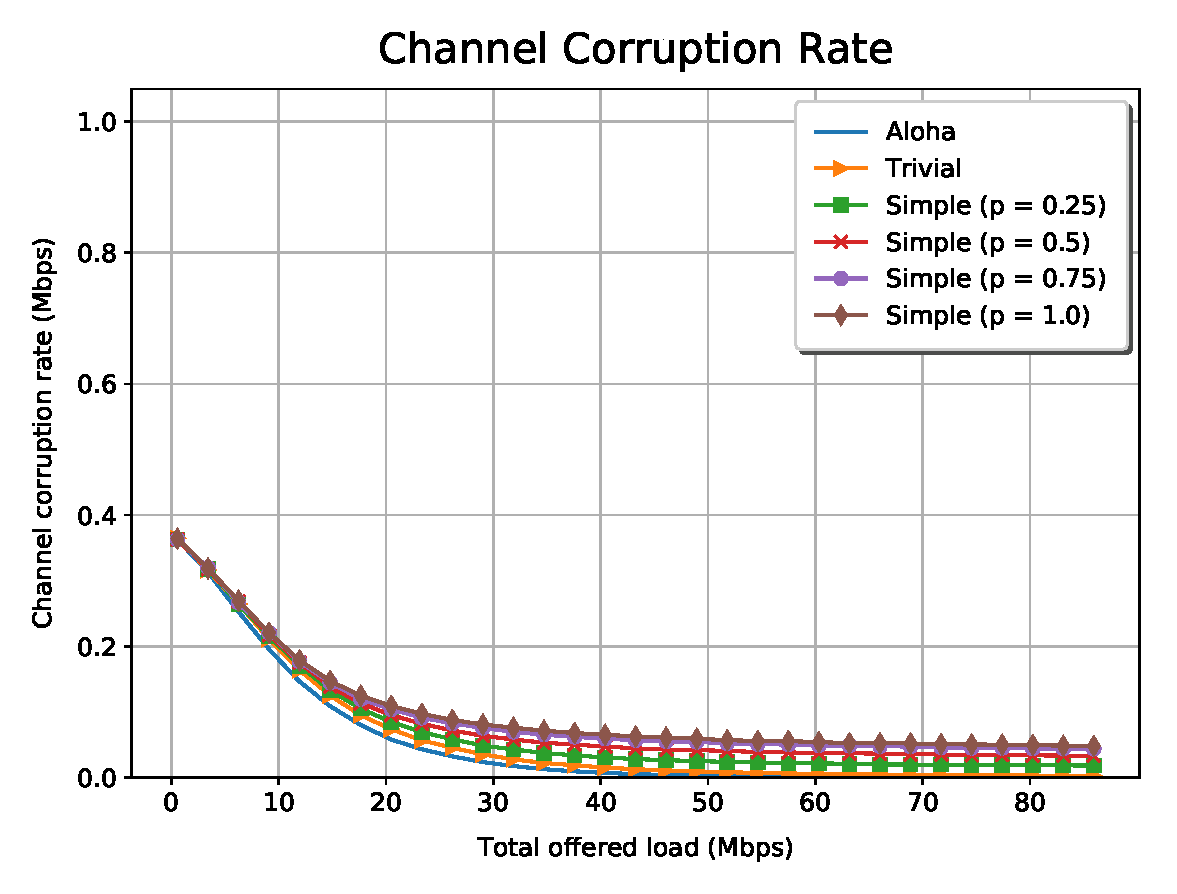
\includegraphics[width=\columnwidth]{figures/plots/realistic_cc}
	\caption{Channel Corruption Rate of the different simulations with respect to the total load on the channel. With high loads, the packets propagation model becomes less important.}
	\label{fig:cc}
\end{figure}


In this section, we compare the different variants of the protocol.
Unless otherwise specified, the results refer to the realistic propagation model.

\subsection{Protocol}
\cref{fig:tr} show that Simple Carrier Sensing performed better then Trivial Carrier Sensing, which performed better than Aloha in terms of throughput.
The increase in throughput is related to the reduction of collisions: indeed, it is easy to see in \cref{fig:cr}  that collision rate of Aloha saturates and Trivial Carrier Sensing tends to \num{1} much quicker than Simple Carrier Sensing.
Simple Carrier Sensing strategy to avoid collisions seems to be more effective then the Trivial one, which in turn is better then Aloha.
In particular, the strategy of Trivial Carrier Sensing is not effective, since all stations will start to transmit together as soon as the channel is free.
The random nature of Simple Carrier Sensing helps to reduce this effect.
The packet drop rate metric confirm this statement: Simple Carrier Sensing has a higher drop rate, which indicate a higher average waiting time to transmit a packet.
When the channel is saturated, most packets are dropped at the sender.


This phenomena is confirmed by the drop rate metric showed in \cref{fig:dr}.
Aloha never senses the channel before transmitting, thus its drop rate increases much slower then Trivial and Simple Carrier Sensing.
On the contrary, with high loads the channel is saturated and most stations are stuck waiting for the channel to be free: most packets are do not fit the limited queue of the stations and are dropped at the sender.

It is interesting to observe the channel corruption rate, showed in \cref{fig:cc}.
With high loads, only a smaller percentage of the packets is corrupted because of the realistic propagation model used.
Most packets are corrupted by collisions.


\subsection{Persistence}
The behaviour of Simple Carrier Sensing is highly dependent of the parameter $p$ used for the persistence.
When $p$ tends to \num{1}, Simple Carrier Sensing behaves exactly like Trivial Carrier Sensing.
When $p$ tends to \num{0}, Simple Carrier Sensing will always wait a random exponential time before transmitting a packet if the channel is occupied.
For intermediate values of $p$, the behaviour is a mixture.
\cref{fig:tr} shows the throughput for different values of $p$: with the given network, higher values of $p$ correspond to a higher throughput.


\subsection{Propagation Model}
The propagation model does not influence the performances of the protocols with respect to the original Aloha.
In fact, the simulations run with the realistic propagation model show exactly the same results as the realistic model.
The throughput for the disk model is about the double of the realistic model.
